\documentclass[12pt,letter]{amsart}
%\usepackage[dvips]{graphics}
\usepackage{epsfig}
\usepackage{graphics}
\usepackage{graphicx}
\usepackage{caption}
%\usepackage{vruler}


\parindent0.5cm

\oddsidemargin1mm\evensidemargin1mm
 \topmargin-5mm
\textheight240mm\textwidth160mm

\def\baselinestretch{1.1}
\newcommand{\ignore}[1]{}
\newcommand{\df}[0]{{\,\rm d }}
\newcommand{\vectpsi}[0]{\mbox{\boldmath $\psi$}}
\newcommand{\vecttau}[0]{\mbox{\boldmath $\tau$}}
\newcommand{\T}[0]{{\bf T}}
\newcommand{\A}[0]{{\bf A}}
\newcommand{\B}[0]{{\bf B}}
\newcommand{\I}[0]{{\bf I}}
\newcommand{\z}[0]{{\bf z}}
\newcommand{\x}[0]{{\bf x}}
\newcommand{\e}[1]{{\bf e}_#1}
\newcommand{\one}[0]{{\bf 1}}
\newcommand{\diag}[1]{{\rm \bf diag}(#1)}

\renewcommand{\thesection}{\Alph{section}}
\pagestyle{plain}


\DeclareCaptionLabelFormat{sfig}{#1 S#2}
\captionsetup[figure]{labelformat=sfig}

\begin{document}

%\advance\textwidth 3cm


\vspace*{-7mm}

\title{Waggle dance distributions quantify collective foraging in honey bee colonies: Supplementary material}
%\author{}
\maketitle

%\begin{center}
%authors,  Vincent A.A. Jansen
%\vspace*{7mm}
%{\bf title}
%\vspace*{11mm}
 %{\bf \underline{Online Supplementary Text and Methods}}
%\end{center}
%\vspace*{11mm}
%\pagebreak
%\setvruler [][][][][][\textwidth]


\section*{The derivation of the full model for the distribution of distances on the dance floor. }

We will build a simple model to describe the distribution of distances reported on the dance floor. We assume that there are $n$ different resources and they are distributed according to a spatial Poisson point process. The Poisson point process places food sources randomly in the environment of the hive with intensity $\lambda_i$ for resource $i$. The quality of that resource we will denote $q_i.$ For convenience, we will order the resources $q_i$ from small to large such that $q_j \ge q_i$ if $j>i$, and $q_n$ is the resource with the highest quality, which we assume is always present in the environment, hence $\lambda_n>0$, and has a resource quality exceeding unity, hence $q_n>1$. Under this ordering, we define $m$, for which $1\le m\le n$, as the lowest index for which $q_m>1$ hence, $q_i<1$ for all $i=1, \dots, m-1$

\subsection*{The distribution of scout dances}

As a scout travels a small distance $\df x$ its search will cover an area $c_s \df x.$ The constant $c_s$ depends on width of the area scanned, the detection rate and the degree to which a the forager's path covers new ground. If we incorporate these factors into the constant $c_s$ the intensity of discovering a resource over a path of distance $\df x$ is  $c_s \df x$. The probability density of $x$, the distance travelled after which the first source is discovered follows a distribution
$$\lambda_s e^{-\lambda_s x}$$
where $\lambda_s= c_s\sum_{i =1}^n\lambda_i.$

The profitability, which depends on quality and distance, of the source dictates the number of repeats of the dance.
What is the distribution of dances on the dance floor?  Let's assume that there is a function that translates the profitability into the expected number of runs of the waggle dance, $\phi(q_i, x)$,  which is a function of quality an distance. We assume that if this function has a non-zero value it decreases with distance, and increases with quality, hence $\frac{\partial \phi(q, x) }{\partial q}>0$ and $\frac{\partial \phi(q, x) }{\partial  x}<0$ if $\phi(q,x)>0$. There is a minimum quality level of the resource that elicits dancing, and we have set this level to unity, such that if $q \le 1$ then $\phi(q, x)=0$ for $x \ge 0$. It follows that for each $q_i>1$ there is a maximum distance $x_{i, {\rm max}}>0$ for which bees do not dance, that is $\phi(q_i, x)=0$ for $x \ge x_{i, {\rm max}}.$

The expected number of dances for a resource of type $i$ located at distance $x$ is $c_s \lambda_i \phi(q_i, x) e^{-\lambda_s x}.$ The expected total number of scout waggle dances on the dance floor is given by $$M_s=\sum_{i=m}^n \int_{0}^\infty \frac{c_s \lambda_i}{\lambda_s} \phi(q_i, x) \lambda_s e^{-\lambda_s x} \df x
$$ and the distribution of scout dances is
$$\frac{\lambda_s e^{-\lambda_s x}\sum_{i=m}^n  \frac{c_s \lambda_i}{\lambda_s} \phi(q_i, x)  }{M_s}
$$

If the bees go out, scout for resources and dance for them this, and there is no further processing of information, this would be the distribution one would expect.

\subsection*{The distribution of recruit dances}

First, we consider a simple scenario and we assume that all resources are of equal quality $q$ with $q>1$. The scouts that report back on the dance floor cover the surroundings of the hive in their forays. How well they cover, depends on the number of scouts, how well their collective paths cover the area and chance of discovery of an item. Let the fraction of sources that can be discovered by the collection of scouts be $c_r$. We assume $0\le c_r \le 1.$

The chance of discovering food source within a radius of $x$ is $e^{-c_r\lambda_r\pi x^2}$, where $\lambda_r= \sum_{i=1}^n \lambda_i  $ and therefore the chance of having the nearest food source that the recruits report is least a distance $x$ away is $P(\underline x \ge x)=e^{-c_r\lambda_r \pi x^2}.$ The distribution of the nearest food source that recruits report is $$2 c_r\lambda_r \pi x e^{-c_r\lambda_r \pi x^2}.$$ The distribution of recruit dances on the dance floor is:
$$\frac{\phi(q,x)2 c_r\lambda_r \pi x e^{-\lambda_r \pi x^2}}{M_r}$$ where
$$M_r=\int_0^\infty \phi(q,x)2c_r \lambda_r \pi x e^{-c_r\lambda_r \pi x^2} \df x.$$

If the resources differ in quality, the same rationale can be applied. Consider two locations that differ in resource quality and distance, the hive can prefer the further location if it is sufficiently better. Likewise, it can prefer a lesser quality location if it is sufficiently nearer. Given that the hive has found a resource at distance $x$ of quality $q_i$ we define a threshold distance $\xi_{ij}(x)$ at which a resource of type $q_j$ has the same profitability. If  $q_j \ge q_i,$ and $0 \le  x \le x_{i,\max}$ then $\xi_{ij}(x)$ satisfies
\begin{equation*}
\left \{
\begin{array}{ll}
\phi(q_i,x)=\phi(q_j, \xi_{ij}(x)) & \text{if }0 \le  x<x_{i,\max}\\
\xi_{ij}(x_{i,\max})=x_{j,\max} & \text{if } x= x_{i,\max}
\end{array}
\right.
\end{equation*}
If  $q_j<q_i,$ and $x<x_{i,\max}$ then $\xi_{ij}$ satisfies
\begin{equation*}
\left \{
\begin{array}{ll}
\xi_{ij}(x)=0& \text{if } 0 \le x \le \xi_{ji}(0) \\
\phi(q_i,x)=\phi(q_j, \xi_{ij}(x)))& \text{if } \xi_{ji}(0)<x_{i,\max}\\
\xi_{ij}(x_{i,\max})=x_{j,\max} & \text{if } x= x_{i,\max}
\end{array}
\right.
\end{equation*}

This relation defines the threshold distance $\xi_{ij}(x)$ as a function of $x$ for $0 \le x \le x_{i,{\rm max}}$.
%It follows from implicit differentiation that if ??? $\frac{\df \xi_{ij}}{\df q_j}=- \frac{\df \phi(q_j,x)/\df q_j}{\df \phi(q,x)/\df x}>0$ and $\frac{\df \xi_{ij}}{\df %q_i}= \frac{\df \phi(q_i,x)/\df q_i}{\df \phi(q,x)/\df x}<0.$
It follows that $\xi_{ii}(x)=x$. Because $\phi(q_i,x)$ increases with $q$ if $\phi(q_i,x)>0$ it follows that $\phi(q_i,x)>\phi(q_j,x)$ if $q_i>q_j$. As a consequence $\xi_{ij}<x$ if $i>j$ and $\xi_{ij}>x$ and if $i<j.$

The probability to find the nearest resource $i$ at distance $x$ is given by the Rayleigh distribution $2 \pi c_r \lambda_i x e^{-\pi c_r \lambda_i x^2 }.$ For $x \le x_{i, {\rm max}}$ the chance of there not being a source if type $j$ within a radius of $\xi_{ij}(x)$, which is $e^{- \pi c_r \lambda_j \xi_{ij}(x)^2}.$ The probability that resource $i$ at location $x$, $0 \le x \le x_{i,\max}$ is the most profitable is therefore
$$P(\textrm{most profitable resource }i \textrm{ is at distance } x)=2 \pi c_r \lambda_i x e^{- \pi \sum_{j=1}^n\lambda_j c_r \xi_{ij}(x)^2}$$ and 0 if $x > x_{i,\max}$
and the probability of finding the most profitable location at distance $x$ is
$$P(\textrm{most profitable resource is at distance } x )=\sum_{\forall i: {x_{i, \max}>x}} 2 \pi c_r \lambda_i x e^{- \pi \sum_{j=1}^n c_r \lambda_j \xi_{ij}(x)^2}.$$
For $x>x_{n, \max}$ the most profitable resource cannot be determined, as all have zero profitability.

The probability of encountering a recruit reporting a distance $x$ on the dance floor is
$$M_r^{-1}\sum_{i=m}^n  \phi(q_i, x)\lambda_i2 \pi c_r  x e^{- \pi \sum_{j=1}^n c_r \lambda_j \xi_{ij}(x)^2}
$$
where $M_r$ is the normalisation factor $$M_r=\int_0^\infty \sum_{i=m}^n  \phi(q_i, x)\lambda_i2 \pi c_r  x e^{- \pi \sum_{j=1}^n c_r \lambda_j \xi_{ij}(x)^2}\df x.$$

\subsection*{The full model}

The combined distribution of distances of scout and recruit dances on the dance floor is given by
$$P(\underline x= x )=p \frac{\lambda_s e^{-\lambda_s x}\sum_{i=1}^n  \frac{c_s \lambda_i}{\lambda_s} \phi(q_i, x) }{M_s} +(1-p)\frac{\sum_{i=1}^n  \phi(q_i, x)2 \pi c_r \lambda_i  x e^{- \pi \sum_{j=1}^n c_r \lambda_j \xi_{ij}(x)^2}}{M_r}.$$
This is a generic model for the distribution of distances reported on the dance floor.

\section*{The simplified model}

The full model can be used to calculate the likelihood for a given data set, which can be used to estimate parameters. The full model has $2 n+ 3 + k $  parameters: $\lambda_1 \dots \lambda_n$, $q_1 \dots q_n$, $c_s, c_r$ and $p$ plus $k$ parameters needed to specify the function $\phi$. Even though it is possible to reduce the number of parameters through a scaling, e.g. by defining $\lambda_i^r=c_r \lambda_i$ and $c=\frac{c_s}{c_r}$, but even if the number of resources is low, it turned out to be difficult to estimate the parameters even if with a fair sized data sets. To assist in the estimation of the key parameters we therefore formulated a simplified model.

We can simplify the model by assuming that the dependence of the number of dances depends less on the distance and more on quality. We assume that that dependence of the profitability assessment only weakly depends on distance and that there is quality differences between resources of a decent size, so that there are a large threshold distances at which resources have the same profitability. If that is the case then, if a resource is discovered at a small distance from the hive, resources if less quality than this one, are not worth dancing for, whereas there is a large distance over which superior resources can be detected that will have higher profitability. In mathematical terms, under this assumption, for small $x$, $\xi_{ij}(x)=0$ if $j<i$, $\xi_{jj}(x)=x$ and $\xi_{ij}(x)$ is large if $j>i$. We thus have $\sum_{j=1}^n  \lambda_j \xi_{ij}(x)=\sum_{j=i}^n  \lambda_j \xi_{ij}(x)$ for $i<n$ and $\sum_{j=1}^n  \lambda_j \xi_{nj}(x)=\lambda_n x.$ Moreover, as the $\xi_{ij}s$ will be large, $\sum_{j=i}^n  \lambda_j \xi_{ij}(x) \gg\lambda_n x.$  We can approximate
$$\sum_{i=1}^n  \phi(q_i,x)2 \pi c_r \lambda_i  x e^{- \pi \sum_{j=1}^n c_r \lambda_j \xi_{ij}(x)^2}\approx
\phi(q_n,x)2 \pi c_r \lambda_n  x e^{- \pi  c_r \lambda_n x^2}
$$
The recruits on the dance floor are most likely to report short distances. By expanding the function $ \phi(q_n, x)$ around $x=0$ we get $\phi(q_n, x)=\left[\phi(q_n, 0)+x\left. \frac{\partial \phi(q_n, x)}{\partial x}\right|_{x=0}+ O(x^2)\right]_+$ we can approximate the recruit distribution as:
$$M_r^{-1}\sum_{i=m}^n  \phi(q_i, x)\lambda_i2 \pi c_r  x e^{- \pi \sum_{j=1}^n c_r \lambda_j \xi_{ij}(x)^2}\approx  \frac{\left[1- a_r x\right]_+2 \pi a_r^2   b_r x e^{- \pi  b_r  (a_r x)^2}}{1-\frac{{\rm erf}\left(  \sqrt{\pi b_r}\right)}{2 \sqrt{b_r }}}$$
with $a_r=-\phi(q_n, 0)^{-1}\left. \frac{\partial \phi(q_n, x)}{\partial x}\right|_{x=0}$ and $b_r=c_r \gamma_n a_r^{-2}$
and where we used
$$\phi(q_n, 0)\int_{0}^{a_r^{-1}} (1- a_r x )2 \pi a_r^2   b_r x e^{- \pi  b_r  (a_r x)^2}\df x=\phi(q_n, 0)\left(1-\frac{{\rm erf}\left(  \sqrt{\pi b_r}\right)}{2 \sqrt{b_r }}\right)
$$ and cancelled the term $\phi(q_n, 0).$

The scouts on the dance floor are more likely to report large distances. For distances around the largest distance for which scouts dance, $x_{n,\max}$, the $\phi(q_i, x)=0$ for all $i<n$. We therefore expand  $ \phi(q_n, x)$ around $x_{n, \max}$ to get $ \phi(q_n, x)=\left[( x- x_{n, \max})\left.\frac{\phi(q_n, x)}{\partial x}\right|_{x=x_{n, \max}}+ O(x^2)]\right]_+$. With this, we can approximate the scout distribution as:
%$$\frac{\lambda_s e^{-\lambda_s x}  \left[  \frac{q_n - 1}{\alpha}-x\right]_+ }{\frac{q_n-1}{\alpha}-\lambda_s^{-1} \left(1-e^{-\lambda_s\frac{q_n-1}{\alpha }}\right)}$$
$$\frac{\lambda_s e^{-\lambda_s x}\sum_{i=m}^n  \frac{c_s \lambda_i}{\lambda_s} \phi(q_i, x)  }{M_s}\approx \frac{a_s b_s e^{-b_s a_s x}  \left[ 1-a_s x\right]_+ }{1-b_s^{-1} \left(1-e^{-b_s}\right)}$$
with $a_s=x_{n,\max}^{-1}$ and $b_s=\gamma_s a_s^{-1}$
and where we used
$$ \frac{c_s \lambda_i}{\lambda_s}\left.\frac{\phi(q_n, x)}{\partial x}\right|_{x=x_{n, \max}} \int_{0}^{a_s^{-1}} a_s b_s e^{-b_s a_s x}  ( 1-a_s x)  \df x= \frac{c_s \lambda_i}{\lambda_s}\left.\frac{\phi(q_n, x)}{\partial x}\right|_{x=x_{n, \max}} \left( 1-b_s^{-1} \left(1-e^{-b_s}\right)\right)$$ and cancelled the term $\frac{c_s \lambda_i}{\lambda_s}\left.\frac{\phi(q_n, x)}{\partial x}\right|_{x=x_{n, \max}}.$

The distribution then simplifies to
$$P(\underline x= x )=p \frac{\left[ 1-a_s x\right]_+a_s b_s e^{-b_s a_s x}   }{1-b_s^{-1} \left(1-e^{-b_s}\right)}+(1-p) \frac{\left[1- a_r x\right]_+2 \pi a_r^2   b_r x e^{- \pi  b_r  (a_r x)^2}}{1-\frac{{\rm erf}\left(  \sqrt{\pi b_r}\right)}{2 \sqrt{b_r }}}.$$
The simplified model has 5 parameters, and is therefore simpler than the full model for $n \ge2$, which has $2+2n+k $ parameters.


\section*{The simplified distribution with a minimum value}
 Let $m$ be the lowest distance that is recorded, for instance because there is a minimum duration of the waggle dance. We assume that $m<\xi_{ji}(0)$ for all $j<i$. For the simplified recruit distribution we now expanding the function $ \phi(q_n, x)$ around $x=m$ to get $\phi(q_n, x)=\left[\phi(q_n, m)+(x-m)\left. \frac{\partial \phi(q_n, x)}{\partial x}\right|_{x=m}+ O(x^2)\right]_+$. The simplified recruit distribution becomes:
%$$\frac{\left[\frac{q_n - 1}{ \alpha q_n}- x\right]_+2 \pi c_r \lambda_n  x e^{- \pi  c_r \lambda_n x^2}}{\left(\frac{ (q_n-1)}{\alpha  q_n}-m\right)e^{-\pi c_r %\lambda_n m^2 }+\frac{\text{erf}\left(m\sqrt{\pi c_r \lambda_n} \right)-\text{erf}\left(\frac{  (q_n-1)}{\alpha  q_n}\sqrt{\pi c_r \lambda_n}\right)}{2 \sqrt{c_r %\lambda_n}}}$$
$$ \frac{\left[1- a_r x\right]_+2 \pi a_r^2 b_r  x e^{- \pi  b_r (a_r x)^2}}{\left(1-a_r m\right)e^{-\pi b_r (a_r m)^2 }+\frac{\text{erf}\left(a_r \sqrt{\pi b_r}m \right)-\text{erf}\left(\sqrt{\pi b_r}\right)}{2 \sqrt{b_r}}}$$
with $a_r=m-\phi(q_n, m)^{-1}\left. \frac{\partial \phi(q_n, x)}{\partial x}\right|_{x=m}$ and $b_r=c_r \gamma_n a_r^{-2}.$

The scout distribution is only affected through the normalisation factor and becomes:
$$
a_s\frac{ b_s e^{-b_s a_s (x-m)}  \left[ 1-a_s x\right]_+ }
{\left(1-a_s m\right)-b_s^{-1}\left(1-e^{-b_s\left(1-a_s m\right)}\right)}$$

The distribution, for $ x \ge m$ then becomes
\begin{eqnarray*}P(\underline x= x )&=&pa_s\frac{ b_s e^{-b_s a_s (x-m)}  \left[ 1-a_s x\right]_+ }
{\left(1-a_s m\right)-b_s^{-1}\left(1-e^{-b_s\left(1-a_s m\right)}\right)}\\&& \qquad +(1-p) \frac{\left[1- a_r x\right]_+2 \pi a_r^2 b_r  x e^{- \pi  b_r (a_r x)^2}}{\left(1-a_r m\right)e^{-\pi b_r (a_r m)^2 }+\frac{\text{erf}\left(a_r \sqrt{\pi b_r}m \right)-\text{erf}\left(\sqrt{\pi b_r}\right)}{2 \sqrt{b_r}}}.
\end{eqnarray*}
The same function describe the distribution of the dance durations, where dances have a minimum duration. This assumes a linear relation between duration and distance.

\section*{Model fits to all sites}

\captionof{table}{Fit results for the fitting of the waggle dance model to each site.}
% latex table generated in R 3.6.3 by xtable 1.8-4 package
% Tue May  3 15:35:09 2022
\scalebox{0.65}{
\begin{tabular}{rllrrrrrrrrrrrrr}
  \hline
 & site & model & loglikelihood & AIC & delta\_AIC & rAIC & wAIC & p & bs & br & as & ar & k & ks\_statistic & ks\_pvalue \\ 
  \hline
1 & BEL & collective & -181.41 & 372.83 & 1.83 & 0.40 & 0.29 & 0.65 & 7.04 & 0.81 & 0.05 & 0.17 &   5 & 0.10 & 0.71 \\ 
  2 & BEL & individual & -183.50 & 371.00 & 0.00 & 1.00 & 0.71 & 1.00 & 4.50 &  & 0.07 &  &   2 & 0.09 & 0.79 \\ 
  3 & BFI & collective & -190.50 & 391.00 & 0.00 & 1.00 & 1.00 & 0.04 & 0.00 & 2.82 & 0.16 & 0.25 &   5 & 0.09 & 0.33 \\ 
  4 & BFI & individual & -211.30 & 426.59 & 35.60 & 0.00 & 0.00 & 1.00 & 9.47 &  & 0.10 &  &   2 & 0.18 & 0.00 \\ 
  5 & BLO & collective & -221.03 & 452.05 & 0.00 & 1.00 & 1.00 & 0.21 & 1.79 & 0.57 & 0.07 & 0.36 &   5 & 0.07 & 0.76 \\ 
  6 & BLO & individual & -237.39 & 478.78 & 26.73 & 0.00 & 0.00 & 1.00 & 5505.00 &  & 0.00 &  &   2 & 0.11 & 0.24 \\ 
  7 & BUR & collective & -118.30 & 246.61 & 0.00 & 1.00 & 1.00 & 0.11 & 0.00 & 500.00 & 0.15 & 0.03 &   5 & 0.07 & 0.82 \\ 
  8 & BUR & individual & -143.72 & 291.44 & 44.83 & 0.00 & 0.00 & 1.00 & 10.00 &  & 0.10 &  &   2 & 0.18 & 0.01 \\ 
  9 & CAD & collective & -48.28 & 106.56 & 2.65 & 0.27 & 0.21 & 0.17 & 0.00 & 0.43 & 1.46 & 0.39 &   5 & 0.08 & 0.95 \\ 
  10 & CAD & individual & -49.95 & 103.91 & 0.00 & 1.00 & 0.79 & 1.00 & 0.00 &  & 0.39 &  &   2 & 0.11 & 0.74 \\ 
  11 & GIL & collective & -74.54 & 159.08 & 0.00 & 1.00 & 1.00 & 0.26 & 0.00 & 0.00 & 0.33 & 0.75 &   5 & 0.14 & 0.06 \\ 
  12 & GIL & individual & -102.31 & 208.62 & 49.53 & 0.00 & 0.00 & 1.00 & 2.04 &  & 0.35 &  &   2 & 0.20 & 0.00 \\ 
  13 & HER & collective & -136.97 & 283.94 & 2.08 & 0.35 & 0.26 & 0.28 & 0.00 & 0.16 & 0.38 & 0.18 &   5 & 0.08 & 0.95 \\ 
  14 & HER & individual & -138.93 & 281.86 & 0.00 & 1.00 & 0.74 & 1.00 & 0.00 &  & 0.18 &  &   2 & 0.11 & 0.59 \\ 
  15 & HHS & collective & -61.35 & 132.70 & 0.00 & 1.00 & 1.00 & 0.10 & 0.00 & 0.00 & 0.14 & 0.50 &   5 & 0.13 & 0.36 \\ 
  16 & HHS & individual & -83.75 & 171.50 & 38.80 & 0.00 & 0.00 & 1.00 & 7.10 &  & 0.13 &  &   2 & 0.24 & 0.01 \\ 
  17 & HOR & collective & -40.50 & 91.00 & 0.00 & 1.00 & 1.00 & 0.06 & 0.00 & 0.54 & 0.22 & 0.63 &   5 & 0.05 & 0.97 \\ 
  18 & HOR & individual & -56.65 & 117.30 & 26.30 & 0.00 & 0.00 & 1.00 & 7.77 &  & 0.20 &  &   2 & 0.17 & 0.02 \\ 
  19 & MAK & collective & -84.52 & 179.04 & 0.00 & 1.00 & 1.00 & 0.21 & 2.32 & 0.02 & 0.12 & 0.48 &   5 & 0.09 & 0.79 \\ 
  20 & MAK & individual & -98.02 & 200.05 & 21.01 & 0.00 & 0.00 & 1.00 & 9.17 &  & 0.10 &  &   2 & 0.19 & 0.03 \\ 
  21 & MEL & collective & -115.32 & 240.63 & 0.00 & 1.00 & 1.00 & 0.08 & 0.00 & 0.00 & 0.21 & 0.34 &   5 & 0.16 & 0.07 \\ 
  22 & MEL & individual & -135.73 & 275.46 & 34.83 & 0.00 & 0.00 & 1.00 & 0.00 &  & 0.25 &  &   2 & 0.24 & 0.00 \\ 
  23 & MPA & collective & -181.87 & 373.75 & 0.00 & 1.00 & 0.96 & 0.57 & 0.58 & 0.00 & 0.19 & 0.42 &   5 & 0.07 & 0.87 \\ 
  24 & MPA & individual & -188.04 & 380.08 & 6.33 & 0.04 & 0.04 & 1.00 & 1.47 &  & 0.19 &  &   2 & 0.10 & 0.43 \\ 
  25 & ROT & collective & -138.13 & 286.26 & 0.00 & 1.00 & 1.00 & 0.31 & 0.00 & 0.00 & 0.31 & 0.48 &   5 & 0.15 & 0.02 \\ 
  26 & ROT & individual & -153.36 & 310.71 & 24.45 & 0.00 & 0.00 & 1.00 & 0.00 &  & 0.35 &  &   2 & 0.20 & 0.00 \\ 
  27 & SAU & collective & -108.18 & 226.37 & 0.00 & 1.00 & 0.99 & 0.31 & 0.00 & 9.98 & 0.26 & 0.16 &   5 & 0.06 & 0.96 \\ 
  28 & SAU & individual & -115.50 & 235.01 & 8.64 & 0.01 & 0.01 & 1.00 & 1.49 &  & 0.27 &  &   2 & 0.13 & 0.21 \\ 
  29 & SOM & collective & -70.54 & 151.07 & 0.00 & 1.00 & 0.96 & 0.00 & 10.00 & 10.00 & 1.50 & 0.15 &   5 & 0.11 & 0.50 \\ 
  30 & SOM & individual & -76.67 & 157.34 & 6.27 & 0.04 & 0.04 & 1.00 & 0.00 &  & 0.38 &  &   2 & 0.16 & 0.10 \\ 
  31 & SRA & collective & -123.37 & 256.74 & 0.00 & 1.00 & 1.00 & 0.24 & 0.00 & 0.21 & 0.21 & 0.49 &   5 & 0.05 & 0.98 \\ 
  32 & SRA & individual & -138.11 & 280.23 & 23.49 & 0.00 & 0.00 & 1.00 & 3.00 &  & 0.21 &  &   2 & 0.14 & 0.07 \\ 
  33 & STU & collective & -155.70 & 321.40 & 4.32 & 0.12 & 0.10 & 0.35 & 0.00 & 1.02 & 0.52 & 0.16 &   5 & 0.05 & 1.00 \\ 
  34 & STU & individual & -156.54 & 317.08 & 0.00 & 1.00 & 0.90 & 1.00 & 1.35 &  & 0.16 &  &   2 & 0.05 & 1.00 \\ 
  35 & SWP & collective & -40.42 & 90.85 & 0.00 & 1.00 & 0.95 & 0.00 & 0.25 & 1.27 & 0.00 & 0.38 &   5 & 0.10 & 0.71 \\ 
  36 & SWP & individual & -46.44 & 96.88 & 6.03 & 0.05 & 0.05 & 1.00 & 0.00 &  & 0.42 &  &   2 & 0.14 & 0.31 \\ 
  37 & YAL & collective & -205.76 & 421.52 & 0.00 & 1.00 & 1.00 & 0.08 & 0.00 & 0.30 & 0.18 & 0.27 &   5 & 0.04 & 0.99 \\ 
  38 & YAL & individual & -222.43 & 448.87 & 27.35 & 0.00 & 0.00 & 1.00 & 0.22 &  & 0.21 &  &   2 & 0.10 & 0.34 \\ 
  39 & ZSL & collective & -110.01 & 230.02 & 0.00 & 1.00 & 1.00 & 0.24 & 0.00 & 0.79 & 0.39 & 0.50 &   5 & 0.04 & 1.00 \\ 
  40 & ZSL & individual & -119.95 & 243.90 & 13.88 & 0.00 & 0.00 & 1.00 & 0.39 &  & 0.42 &  &   2 & 0.10 & 0.25 \\ 
   \hline
\end{tabular}
}


\vspace*{50px}


\begin{figure}[h]
	\centering
	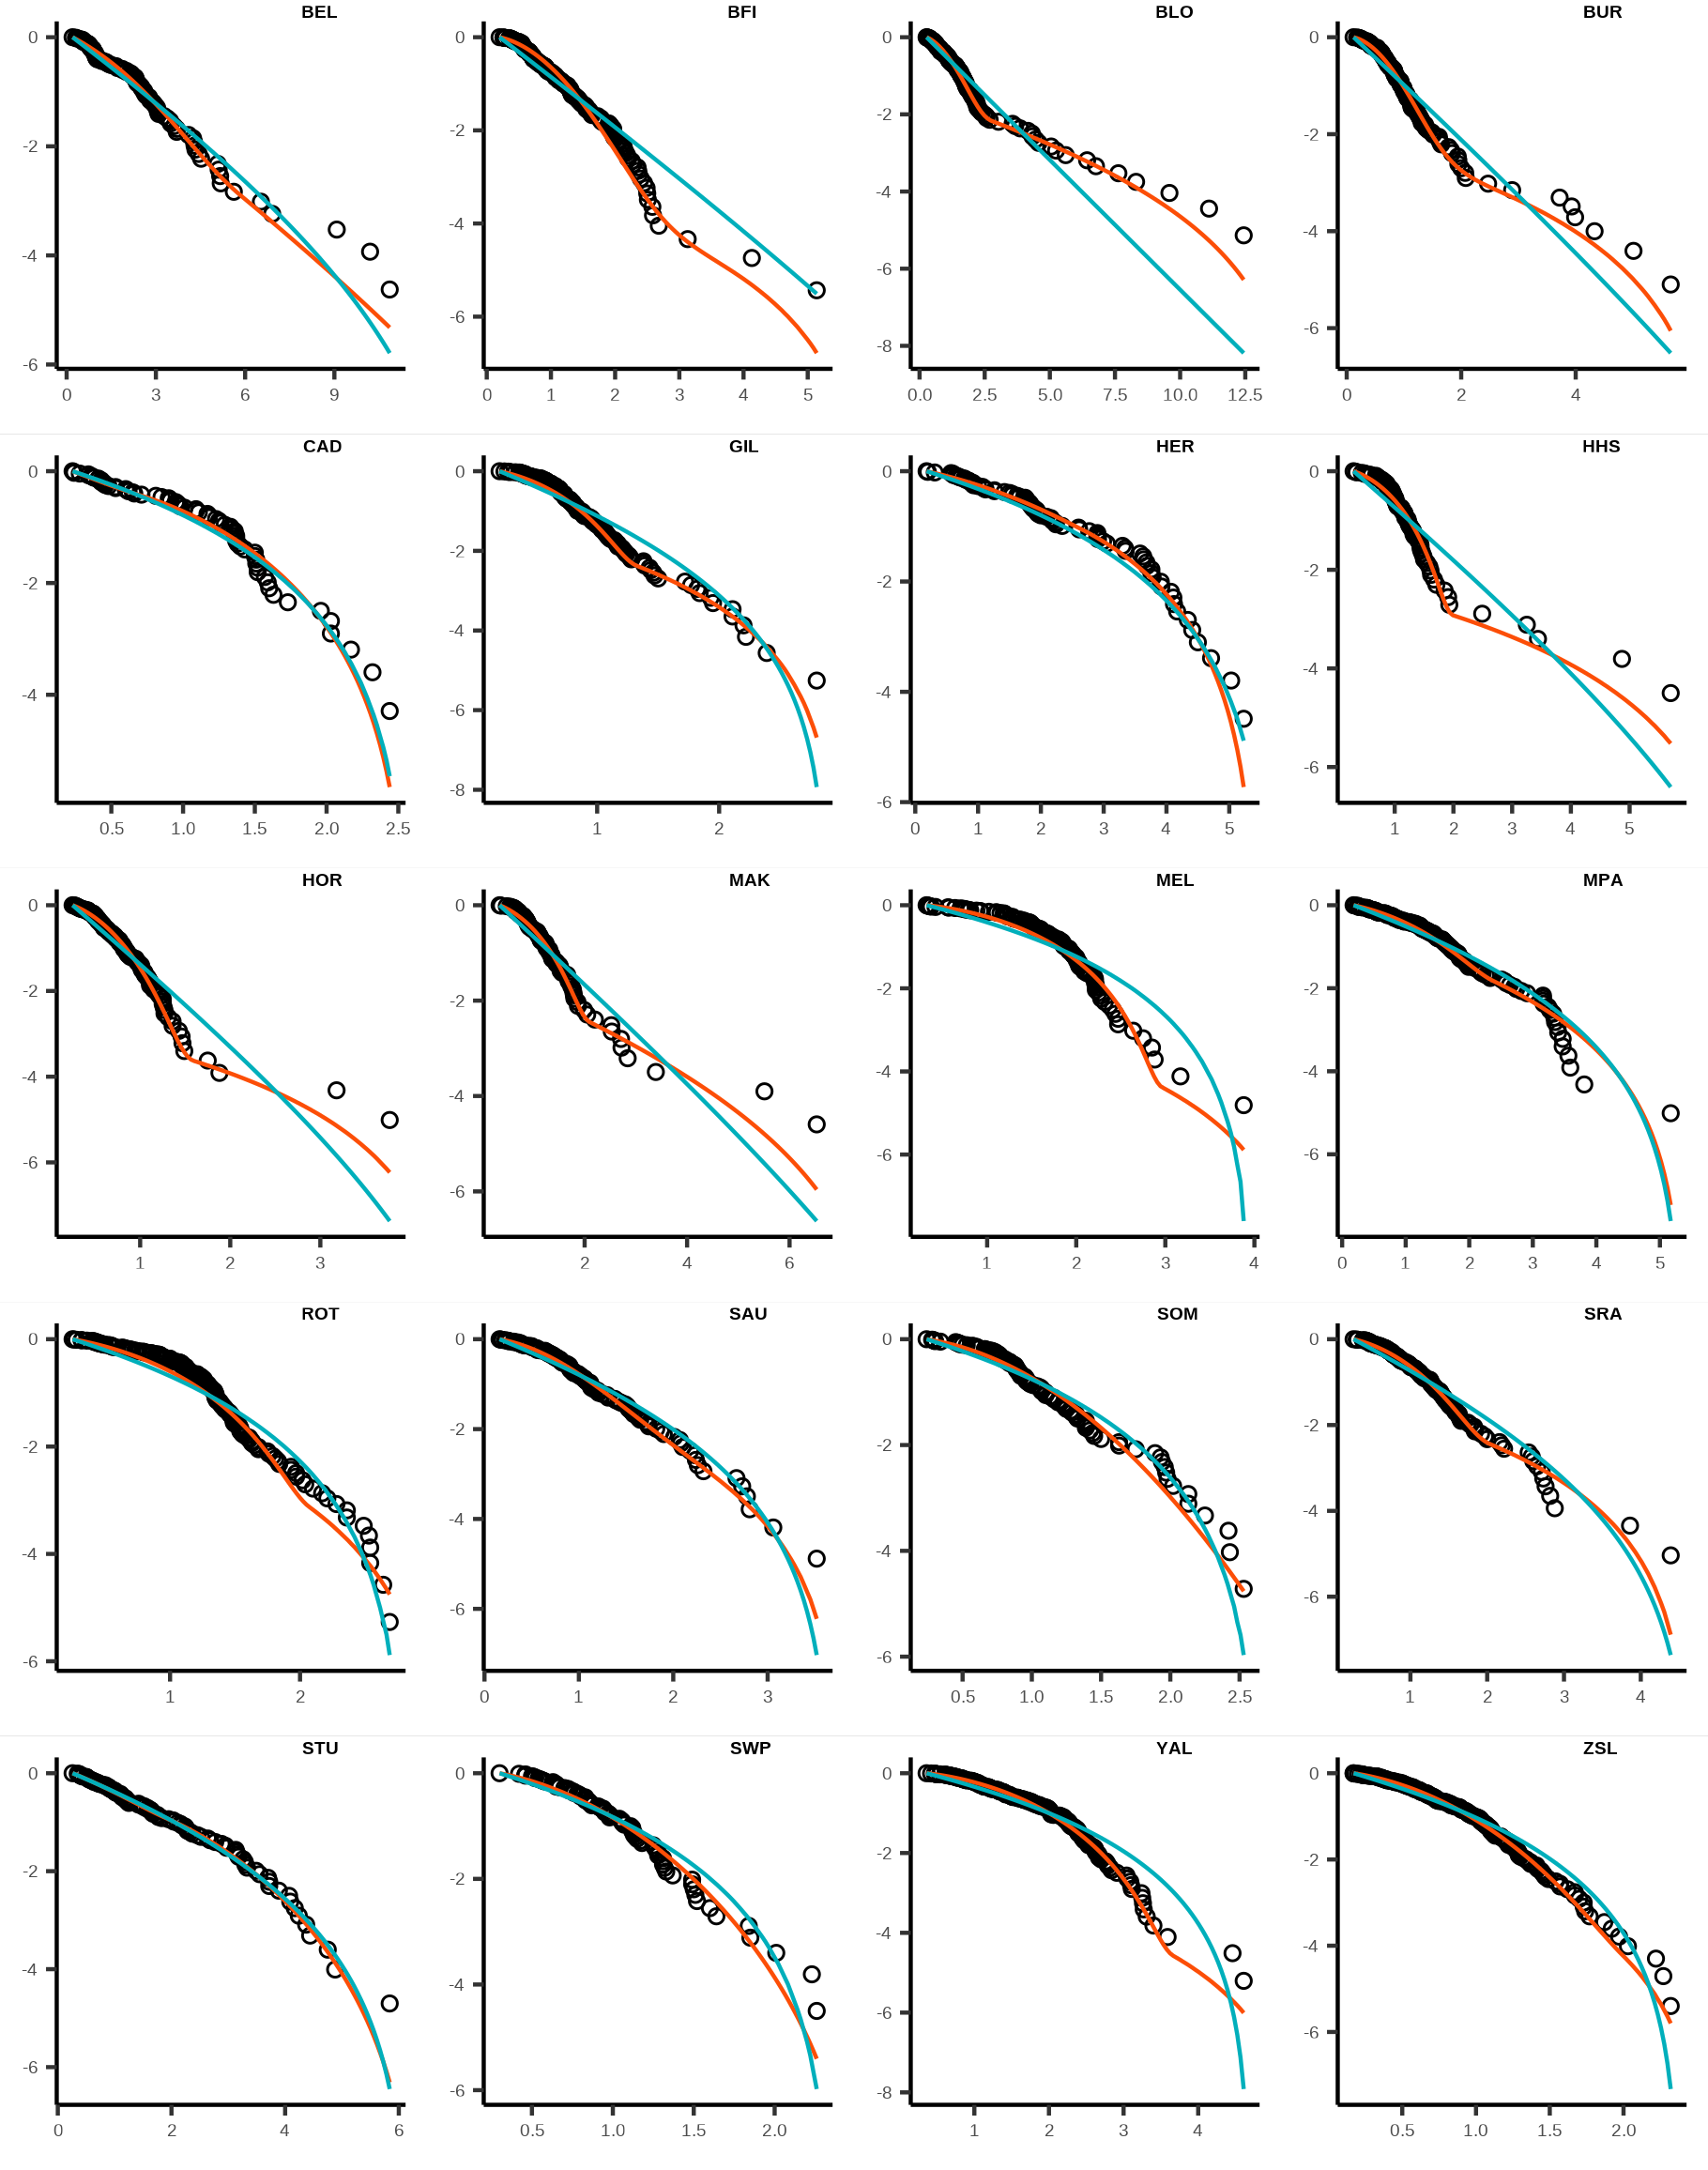
\includegraphics{../results/figures/SI_figures/allsites_plot.png}
	\caption{\textbf{Cumulative frequency distribution} of waggle dance durations and fits of the collective (red line) and individual (blue line) models for all 20 sites}
\end{figure}

\newpage

\section*{Jackknifed partial least squares analysis}

\begin{figure}[h]
	\centering
	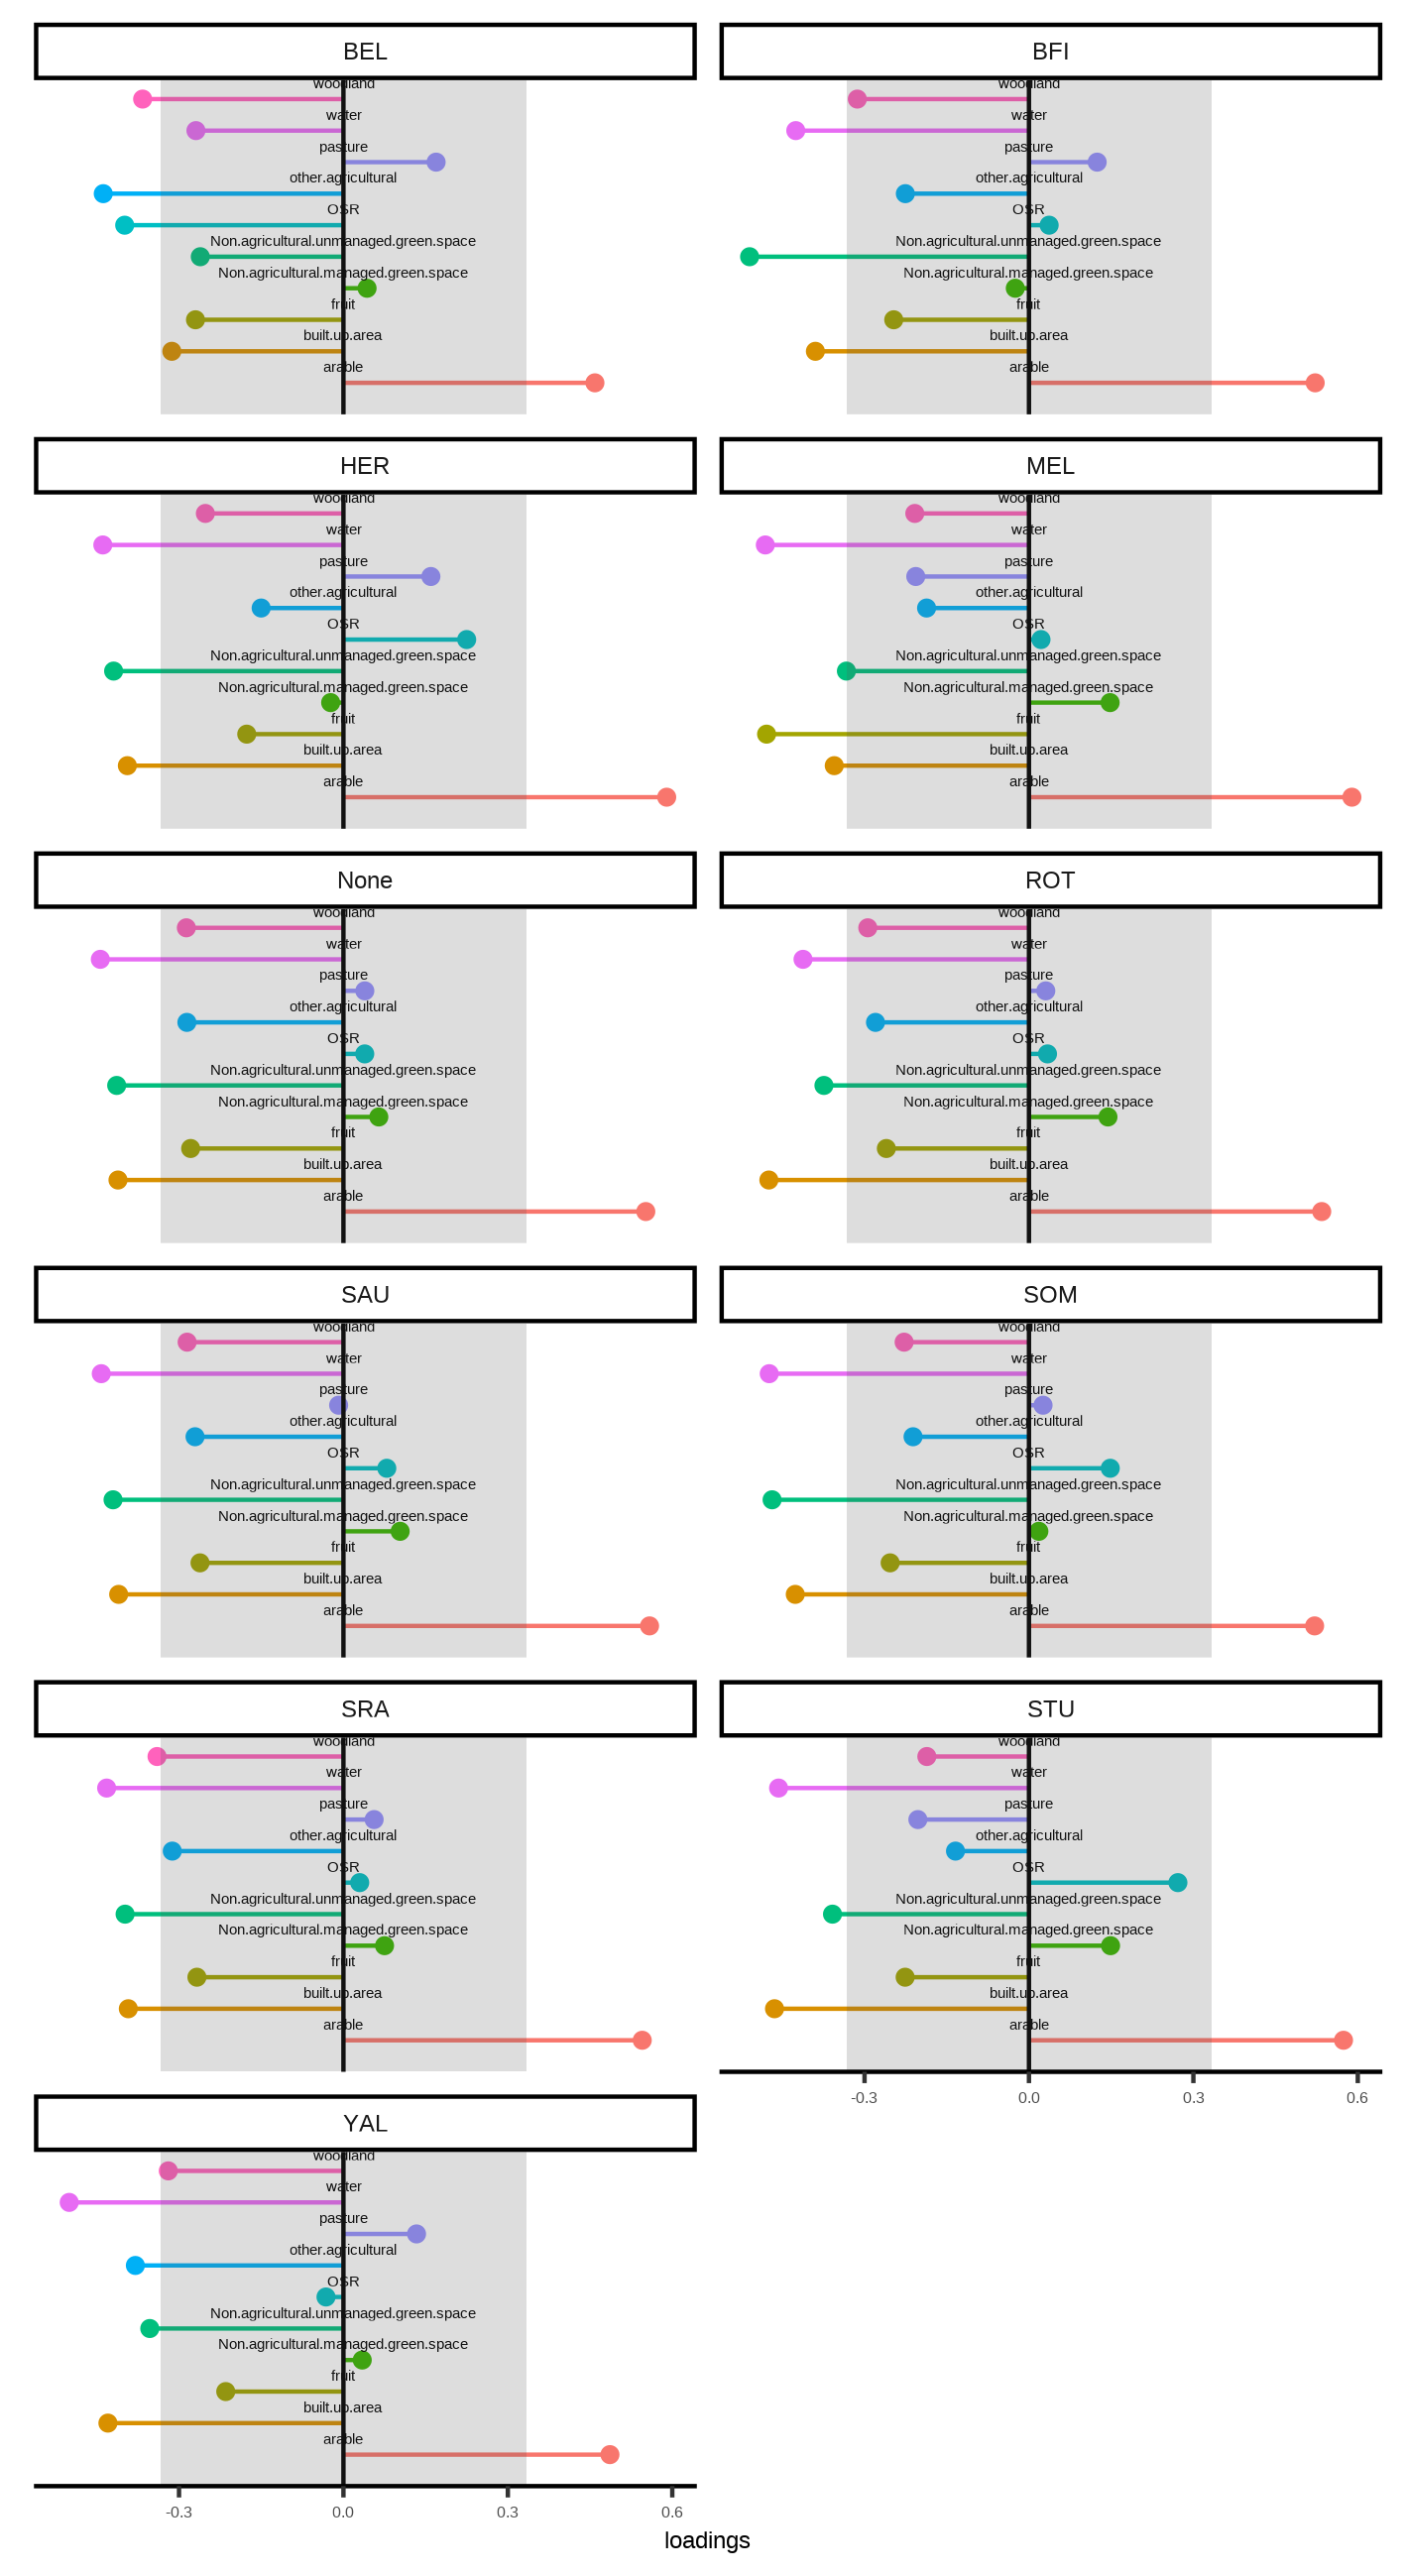
\includegraphics{../results/figures/SI_figures/agrirural_jk_individual_loadings.png}
	\caption{\textbf{Loadings of PLS calculated for each site removed for the agri-rural sites}. Each plot shows the loadings of the first principle component with that site removed from the analysis, showing the individual points making up the overall box plot loadings in Fig 4b.}
\end{figure}

\begin{figure}[h]
	\centering
	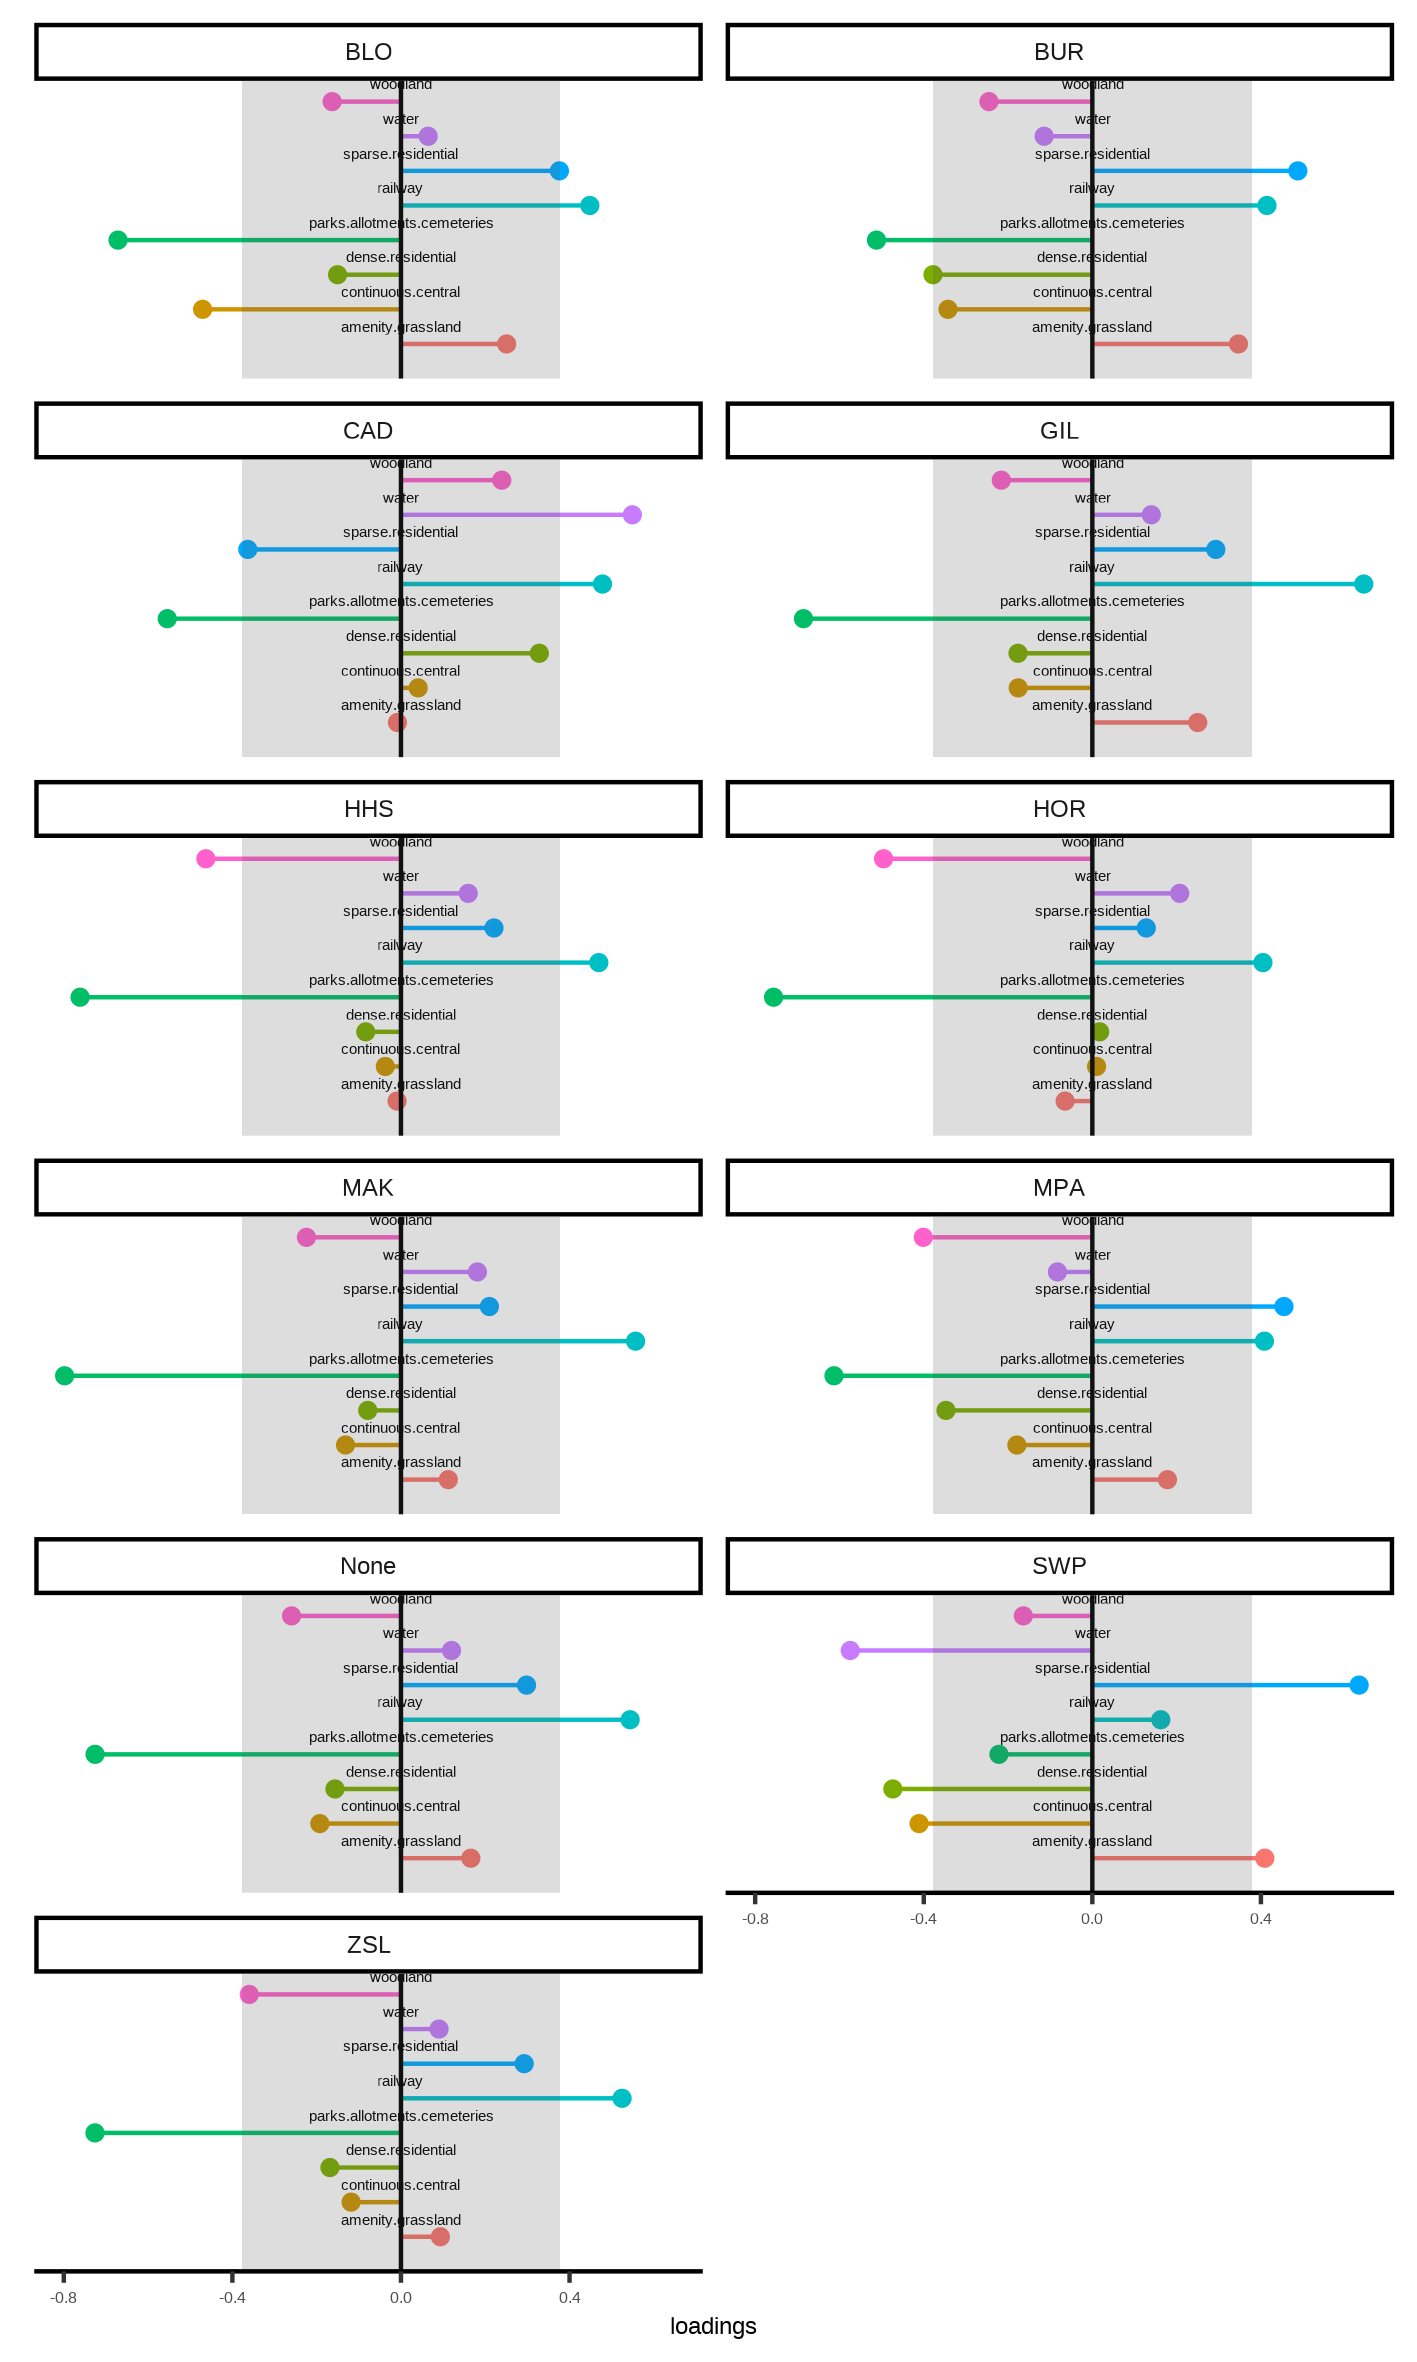
\includegraphics{../results/figures/SI_figures/urban_jk_individual_loadings.png}
	\caption{\textbf{Loadings of PLS calculated for each site removed for the urban sites}. Each plot shows the loadings of the first principle component with that site removed from the analysis, showing the individual points making up the overall box plot loadings in Fig 4d.}
\end{figure}

\end{document}


With the complementary cumulative ($x \ge m$):
\begin{eqnarray*}P(\underline x > x )&=&p\frac{\left(1-a_s x\right)e^{-a_s b_s (x-m)}-b_s^{-1}\left(e^{-a_s b_s(x-m)}-e^{-b_s\left(1-a_s m\right)}\right) }
{\left(1-a_s m\right)-b_s^{-1}\left(1-e^{-b_s\left(1-a_s m\right)}\right)}\\&& \qquad +(1-p) \frac{\left(1-a_r x\right)e^{-\pi b_r (a_r x)^2 }+\frac{\text{erf}\left(a_r \sqrt{\pi b_r}x \right)-\text{erf}\left(\sqrt{\pi b_r}\right)}{2 \sqrt{b_r}}}{\left(1-a_r m\right)e^{-\pi b_r (a_r m)^2 }+\frac{\text{erf}\left(a_r \sqrt{\pi b_r}m \right)-\text{erf}\left(\sqrt{\pi b_r}\right)}{2 \sqrt{b_r}}}.
\end{eqnarray*}

\begin{eqnarray*}P(\underline x > x )&=&p\frac{\left(1-a_s x\right)e^{-a_s b_s x}-b_s^{-1}\left(e^{-a_s b_sx}-e^{-b_s}\right) }
{\left(1-a_s m\right)e^{-a_s b_s m}-b_s^{-1}\left(e^{-a_s b_s m}-e^{-b_s}\right)}\\&& \qquad +(1-p) \frac{\left(1-a_r x\right)e^{-\pi b_r (a_r x)^2 }+\frac{\text{erf}\left(a_r \sqrt{\pi b_r}x \right)-\text{erf}\left(\sqrt{\pi b_r}\right)}{2 \sqrt{b_r}}}{\left(1-a_r m\right)e^{-\pi b_r (a_r m)^2 }+\frac{\text{erf}\left(a_r \sqrt{\pi b_r}m \right)-\text{erf}\left(\sqrt{\pi b_r}\right)}{2 \sqrt{b_r}}}.
\end{eqnarray*}



\section*{Estimating $p$}
The probabilities are of all of the form $P(\underline x= x )=p f(x)+ (1-p) g(x), $ with $f$ and $g$ functions of $x$ that have values between 0 and 1.  The likelihood of the parameter $p$, given a set of data $\x =\{ x_1, \dots, x_n\}$ is
$$L(p|\x)=\prod_{i=1}^n p f(x_i)+ (1-p) g(x_i).$$ If $f(x_i) \ne g(x_i)$ for all $i$, this is a polynomial of degree $n$ (and the degree $n-m$ if there are $m$ elements of $\x$ for which $f(x)= g(x)$. In what follows we will assume that $f(x_i), f(x_i) \ne 0$ and $f(x_i) \ne g(x_i)$ for all $i$. \footnote{It is easy to do the analysis in case there are elements for which $f(x)= g(x)$ by ordering the data points so that for the first $n-m$ elements $f(x_i) \ne g(x_i)$ so that the likelihood can be written as $L(p|\x)=\prod_{i=n-m+1}^n f(x_i) \prod_{i=1}^{n-m} p f(x_i)+ (1-p) g(x_i)$ and follow through the same argument for the $n-m$ roots. } By rewriting the likelihood as
$$L(p|\x)=\prod_{i=1}^n\left(g(x_i)-f(x_i)\right)\prod_{i=1}^n \frac{g(x_i)}{g(x_i)-f(x_i)}-p $$ it is easy to see that the roots of the polynomial are all real valued and take value $\frac{g(x_i)}{g(x_i)-f(x_i)}.$ There are no roots of the polynomial in the interval $[0,1]$: all roots take either negative values, or are larger than 1. This is easy to see: if the root is positive, it requires $g(x)>f(x)$, but this implies that the root must be larger than 1 as $\frac{g(x_i)}{g(x_i)-f(x_i)}=1+\frac{f(x_i)}{g(x_i)-f(x_i)}>1$ if $g(x)>f(x)$.

If $p=0$ the likelihood is given by $L(0|\x)=\prod_{i=1}^n g(x_i)>0. $ Likewise, if $p=1$ the likelihood is given by $L(1|\x)=\prod_{i=1}^n f(x_i)>0. $ As the $L(p|\x)>0$ for all for which $0 \le p \le 1$ the function is continuous, positive on the interval $[0,1].$ The maxima of the likelihood obey $\frac{\df  \mathcal{L}(p|\x)}{\df p}=-\sum_{i=1}^n \left(\frac{g(x_i)}{g(x_i)-f(x_i)}-p\right)^{-1}=0$ where $\mathcal{L}(p|\x)=\ln L(p|\x)$ is the log-likelihood.

The function $\frac{\df  \mathcal{L}(p|\x)}{\df p}$ is a continuously decreasing function of $p$. This follows from the fact that $\frac{\df^2  \mathcal{L}(p|\x)}{\df p^2}=-\sum_{i=1}^n \left(\frac{g(x_i)}{g(x_i)-f(x_i)}-p\right)^{-2}$ which is negative for all values of $p$. As a consequence, on the interval $[0,1]$ there is at most one value for $p$ for which $\frac{\df  \mathcal{L}(p|\x)}{\df p}=0$ and there is a single maximum for the likelihood ${L}(p|\x)$ in $p$. Moreover, if $\left.\frac{\df  \mathcal{L}(p|\x)}{\df p}\right|_{p=0}>0$ and $\left.\frac{\df  \mathcal{L}(p|\x)}{\df p}\right|_{p=1}\ge 0$ the likelihood function is continuously increasing on $[0,1]$ and the maximum is attained for $p=1$. Likewise, if $\left.\frac{\df  \mathcal{L}(p|\x)}{\df p}\right|_{p=0}\le 0$ and $\left.\frac{\df  \mathcal{L}(p|\x)}{\df p}\right|_{p=1}<0$ the likelihood function is continuously decreasing on $[0,1]$ and the maximum is attained for $p=0$. If $\left.\frac{\df  \mathcal{L}(p|\x)}{\df p}\right|_{p=0}>0$ and $\left.\frac{\df  \mathcal{L}(p|\x)}{\df p}\right|_{p=1}<0$ the likelihood function for $p$ attains a single maximum on $(0,1)$.

To find the value of the maximum likelihood, the following methodology can be used:
\begin{itemize}
\item Determine if $f(x_i) \ne g(x_i)$ for any $i$. If so, remove them from the data set and proceed with the remaining $n$ data points.
\item Calculate the derivatives of the log likelihood for $p=0$ and $p=1$. These are given by: $$\left.\frac{\df  \mathcal{L}(p|\x)}{\df p}\right|_{p=0}=-\sum_{i=1}^n \left(\frac{g(x_i)}{g(x_i)-f(x_i)}\right)^{-1}=-n+\sum_{i=1}^n \frac{f(x_i)}{g(x_i)}$$
    $$\left.\frac{\df  \mathcal{L}(p|\x)}{\df p}\right|_{p=1}=-\sum_{i=1}^n \left(\frac{f(x_i)}{g(x_i)-f(x_i)}\right)^{-1}=n-\sum_{i=1}^n \frac{g(x_i)}{f(x_i)}$$
\item If $\left.\frac{\df  \mathcal{L}(p|\x)}{\df p}\right|_{p=0}\le 0$ and $\left.\frac{\df  \mathcal{L}(p|\x)}{\df p}\right|_{p=1}<0$ the maximum is attained for $p=0$
\item If $\left.\frac{\df  \mathcal{L}(p|\x)}{\df p}\right|_{p=0}>0$ and $\left.\frac{\df  \mathcal{L}(p|\x)}{\df p}\right|_{p=1}\ge 0$ the maximum is attained for $p=1.$
\item If $\left.\frac{\df  \mathcal{L}(p|\x)}{\df p}\right|_{p=0}>0$ and $\left.\frac{\df  \mathcal{L}(p|\x)}{\df p}\right|_{p=1}<0$ the likelihood function for $p$ attains a single maximum on $(0,1)$ and can be determined by numerical means such as Newton's method. An obvious initial point for such a method is $p_0=\frac{\left.\frac{\df  \mathcal{L}(p|\x)}{\df p}\right|_{p=0}}{\left.\frac{\df  \mathcal{L}(p|\x)}{\df p}\right|_{p=0}-\left.\frac{\df  \mathcal{L}(p|\x)}{\df p}\right|_{p=1}}$ (which is the intersection with the p-axis of a straightline between the values calculated for $p=0$ and $p=1$).
\end{itemize}



\section*{Seeley's profitability function}

To apply this model to data we will need a detailed description of how bees translate the quality $q$ and distance $x$ of a resource into $\phi(q, x)$, their measure of profitability. Tom Seeley conducted detailed experiments how honey bees respond to differences in quality and distance (REFS).

Seeley's work has shown that bees judge the profitability of a resource by the and optimise the energy efficiency, i.e  the net energy gain per amount of energy spend. Seeley (1994) takes the gain to be proportional to the load carried and the sucrose concentration. The cost depends on the different activities undertaken (e.g. flights in and out, collecting food, unloading food) and the respective times these activities took, and the energy spend in undertaking them.

Let the sucrose concentration be given by $q'$ and the travel distance by $x$. The gain is the $G$ is proportional to the quality, and the cost, $C$, increases linearly with the energy spent. We assume here that energy spent is fixed costs and further increases linearly with distance. We can then write the net energy efficiency as
$\frac{G-C}{C}= \frac{q}{1+\alpha  x}-1, $ where $q$ is the quality of the resource and $\alpha$ the energy spend per distance, and both measures are taken relative to the fixed cost of travel.
 If we assume that the bees do not dance if the profitability is negative, we as a measure for the propensity of bees to dance in relation to resource quality and distance the function:
$$\phi(q,x)=\left[\frac{q}{1+\alpha x}-1\right]_+$$
 (we used the notation $[x]_+=\max(x,0)$).
This function has the property that for a fixed $x$, there is a minimum quality $q=1+\alpha  x$ below which the bees don't dance (compare to Fig 5:10, Seeley (1984)). The equivalent quality for two resources at distances $x_1$ and $x_2$ is $\frac{1+\alpha x_2}{1+\alpha x_1}=\frac{ q_2}{q_1}$; the equivalent quality increases linearly with distance (more or less born out by Boch 1956). The critical distance $\xi_{ij}$ is given by $ \xi_{ij}=\left[\frac1 \alpha\frac{ q_j-q_i}{q_i}+ \frac{ q_j}{q_i}x\right]_+.$

The representation of distances on the floor then follows the distribution:
$$P(\underline x= x )=p \frac{\lambda_s e^{-\lambda_s x}\sum_{i=m}^n  \frac{c_s \lambda_i}{\lambda_s} \left[\frac{q_i}{1+\alpha x}-1\right]_+ }{M_s} +(1-p)\frac{\sum_{i=m}^n  \left[\frac{q_i}{1+\alpha x}-1\right]_+2 \pi c_r \lambda_i  x e^{- \pi \sum_{j=1}^n c_r \lambda_j \xi_{ij}(x)^2}}{M_r}$$
with $$M_s=\sum_{i=m}^n \int_{0}^{\frac{q_i-1}{\alpha}} \frac{c_s \lambda_i}{\lambda_s} \left(\frac{q_i}{1+\alpha x}-1\right) \lambda_s e^{-\lambda_s x} \df x
$$ and
$$M_r= \sum_{i=m}^n \int_0^{\frac{q_i-1}{\alpha}} \left(\frac{q_i}{1+\alpha x}-1\right)\lambda_i2 \pi c_r  x e^{- \pi \sum_{j=1}^n c_r \lambda_j \xi_{ij}(x)^2}\df x.$$


This model can be used to calculate the likelihood for a given data set. In the likelihood calculation the  normalisation factors can be calculated numerically for a given set of parameters. As the same normalisation factor applies to all data points, this is not a very computationally intensive procedure.

This model has $2 n+ 4 $ parameters but contains a redundant parameter:
By defining $\lambda_i^r=c_r \lambda_i$ and $c=\frac{c_s}{c_r}$ the number of parameters can be reduced by one. Alternatively, the parameter $c_r$ can be set to 1 without loss of generality to reduce the number of parameters to $2n+ 3. $

The Seeley model provides a biologically grounded description of the distribution of dances on the dance floor. It contains a large number of parameters, and in many practical applications it is challenging to determine all parameters as the model is ill conditioned: the model tends to give the same or very similar behaviour for a certain combinations of parameters. This makes it difficult or impossible to estimate the value parameters of interest with an accuracy. We will next consider a number of other models that are simplifications of the above model. Three simple and straightforward cases are:
\begin{itemize}
\item Scouts only: $p=1$ (tantamount to saying the colony does not act as a superorganism, the information on the dance floor is scouts information pooled, but not processed)
\item Recruits only: $p=0$ (tantamount to saying each forager can take the same decisions as the hive can. The colony does not act as a superorganism because the capabilities of the dance floor do not exceed that of the individual)
\item One resource only: $n=1$
\item No dependence on distance: $\alpha \rightarrow 0$
\end{itemize}
If the profitability becomes independent of distance the pdf reduces to:
$$\lim_{\alpha \rightarrow 0} P(\underline x= x )=p \lambda_s e^{-\lambda_s x} +(1-p)  2 \pi c_r \lambda_n  x e^{- \pi c_r \lambda_n x^2}$$
where we assumed the for the best resource $q_n>1.$ Also in this case there is a redundant parameter and  $c_r$ can be set to 1 without loss of generality.

\section*{The most profitable resource distribution }
 (to be suppressed, but just in case)
The probability of finding the most profitable resource at a distance  $0 \le x \le x_{n, {\rm max}}$ is a proper probability distribution.
This is because $$\int_{0}^\infty  \sum_{\forall i: {x_{i, \max}>x}}^n 2 \pi c_r \lambda_i x e^{- \pi \sum_{j=1, }^n c_r \lambda_j \xi_{ij}(x)^2}\df x=1- \int_{x_{n, \max}}^\infty  2 \pi c_r \lambda_n x e^{- \pi  c_r \lambda_n x^2}\df x$$

To show this, we first establish that \begin{equation}\xi_{ij}(\xi_{ki}(x))=\xi_{kj}(x) \label{phiresult}.\end{equation} Note that $\phi(q_k,x)=\phi(q_i,\xi_{ki}(x))=\phi(q_j,\xi_{ij}(\xi_{ki}(x)))$ From the definition of $\phi$ it follows that $\phi(q_k,x)=\phi(q_j,\xi_{kj}).$ From this (\ref{phiresult}) follows.
As a corollary, $\xi_{ij}(\xi_{ji}(x))=x$ and hence the function $\xi_{ij}(x)$ is the inverse of $\xi_{ji}(x)$.

Because we order the $q_i$ from small to large, and because $\xi_{ij}$ increases with $q_j$, and decreases with $q_i, $ $\xi_{ij}(x)>\xi_{ji}(x)$ if $i<j$.

We evaluate the integral
\begin{eqnarray*}&&\int_{0}^\infty  \sum_{\forall i: {x_{i, \max}>x}}^n 2 \pi c_r \lambda_i x e^{- \pi \sum_{j=1}^n c_r \lambda_j
\xi_{ij}(x)^2}\df x\\
&=& \sum_{i=1}^n \int_{0}^{x_{i, \max}}  2 \pi c_r \lambda_i x_i e^{- \pi \sum_{j=1}^n c_r \lambda_j
\xi_{ij}(x_i)^2}\df x_i\\
\end{eqnarray*}
substitute $x=\xi_{in}(x_i)$, $x_i=\xi_{ni}(x)$, $\df x_i=\xi_{ni}'(x) \df x$
\begin{eqnarray*}
&=& \sum_{i=1}^n \int_{0}^{x_{n, \max}}  2 \pi c_r \lambda_i \xi_{ni}(x)\xi_{ni}'(x) e^{- \pi \sum_{j=1}^n c_r \lambda_j
\xi_{ij}(\xi_{ni}(x))^2} \df x\\
&=& \int_{0}^{x_{n, \max}}  2\pi\sum_{i=1}^n   c_r \lambda_j \xi_{ni}(x)\xi_{ni}'(x) e^{- \pi \sum_{j=1}^n c_r \lambda_j
\xi_{nj}(x)^2} \df x\\
&=&1- \int_{x_{n, \max}}^\infty  2 \pi c_r \lambda_n x e^{- \pi  c_r \lambda_n x^2}\df x
\end{eqnarray*}
q.e.d

------

\end{document}
